\chapter{Marco teórico}
\label{cap:marco}

La medición de un pez a partir de una fotografía tomada a través de un vidrio requiere encadenar varias etapas, y cada una de ellas puede introducir error. En primer lugar es necesario definir qué se mide y contra qué referencia física; luego, comprender cómo se forma la imagen cuando la luz atraviesa el agua, el vidrio y el aire; y finalmente marcar los puntos anatómicos, recuperar la escala y comparar lo estimado con lo medido. Las etapas de esa cadena se muestran en la Figura~\ref{fig:2-1}, en el mismo orden en que las desarrolla el marco referencial de este capítulo.

Este capítulo tiene tres partes. Primero se revisan los antecedentes y, a partir de ellos, se identifica la brecha que motiva el trabajo (\ref{sec:antecedentes}). Después se desarrolla la teoría de cada etapa de la cadena de medición (\ref{sec:referencial}). Al final se definen los términos que se usan a lo largo del documento (\ref{sec:conceptual}).

\begin{figure}[H]
\centering
\caption[Flujo teórico simplificado de la investigación]{Flujo teórico simplificado de la investigación: escena y referencia física, formación refractiva de la imagen, marcado manual único de puntos, comparación de las rutas A, \Aprime, B y C y evaluación con profundidad conocida o desconocida.}
\label{fig:2-1}
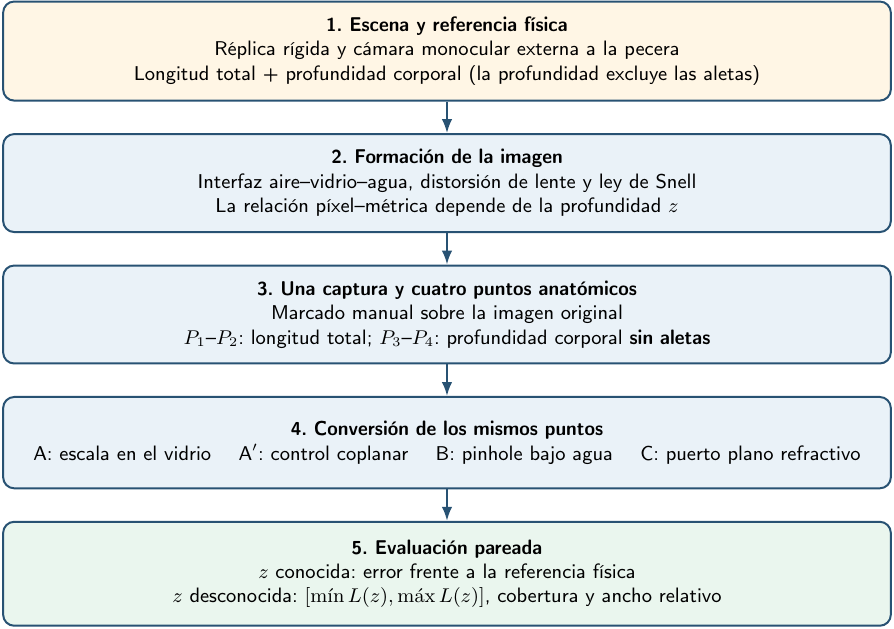
\includegraphics[width=0.85\textwidth]{fig2_1_flujo.png}
\fignota{Elaboración propia.}
\end{figure}

\section{Antecedentes}
\label{sec:antecedentes}

Se realizó una revisión narrativa estructurada de los trabajos sobre medición morfométrica con imágenes, marcado manual o localización de puntos anatómicos, recuperación de escala y formación de imágenes a través de medios refractivos. La búsqueda comenzó con términos generales como «fish measurement», «morphometric analysis», «fish size estimation», «non-invasive measurement» e «image processing», y continuó con combinaciones más específicas: «underwater fish length measurement», «fiducial marker fish measurement», «ArUco fish length», «flat-port camera», «air-glass-water refraction», «refractive camera calibration» y «refraction-aware fish measurement». Las bases consultadas fueron Semantic Scholar y Google Scholar, y la búsqueda se completó siguiendo las referencias de los trabajos encontrados y revisando las fuentes originales. Dado que no se aplicó un protocolo exhaustivo de selección y exclusión, la revisión se considera narrativa y no sistemática. La búsqueda se cerró en septiembre de 2026. Se incluyeron trabajos en español o inglés que trataran al menos uno de estos temas: medición morfométrica de peces con imágenes, recuperación de escala o de puntos anatómicos, calibración de cámaras a través de interfaces aire--vidrio--agua, o modelos explícitos de refracción aplicables a un montaje acuático. Se excluyeron los trabajos sin relación con la medición de organismos acuáticos, la calibración óptica, el marcado de puntos o la estimación de escala, los duplicados y los documentos cuya fuente primaria no pudo identificarse. Además de los catorce trabajos que resume la Tabla~\ref{tab:antecedentes}, se examinaron alrededor de veinte resultados que no se incorporaron a esa matriz.

\textcite{Petrtyl2014} midieron 18 caracteres morfométricos de carpa prusiana de dos maneras, con calibre digital y sobre imágenes, y repitieron las medidas con dos investigadores. Los sesgos relativos medios fueron de $-4{,}27$~\% a $9{,}48$~\%, y en varias comparaciones las diferencias resultaron significativas. Es decir, ni la medición manual ni la digital están libres de sesgo, y ambas cambian según quién mide y cuántas veces. Por eso en este trabajo la referencia manual se tomó con un procedimiento fijo y se la trata como una medida con su propia incertidumbre, no como el valor verdadero.

Sobre la automatización de la información anatómica, \textcite{Petrellis2021} combinó procesamiento de imágenes, detección de contornos, correspondencia de patrones y aprendizaje profundo para estimar la longitud, la profundidad corporal y el área en términos relativos, y para localizar aletas y otras regiones. El error en longitud se ubicó entre 1,9~\% y 13,2~\%. El método trabajó sobre todo con dimensiones relativas, y \citeauthor{Petrellis2021} propuso pasar a visión estéreo, es decir, dos cámaras que observan la misma escena y permiten calcular por triangulación la distancia de cada punto \parencite{Hartley2004}, para obtener dimensiones absolutas en peces inclinados u ocultos.

\textcite{Saleh2023} propusieron MFLD-net, una red liviana que detecta 16 puntos anatómicos en imágenes de peces y, a partir de ellos, calcula la longitud total, la longitud estándar, la longitud cefálica y la profundidad corporal. El modelo logró una precisión promedio de detección $\mathrm{AP} = 0{,}967$ y errores absolutos medios de 9,25~mm en longitud total, 8,27~mm en longitud estándar, 6,57~mm en longitud cefálica y 7,62~mm en profundidad corporal. De este trabajo se tomaron las definiciones de los extremos anatómicos. Su montaje, con cámara industrial y cinta transportadora, es distinto del de esta tesis, donde la imagen se forma a través del vidrio y del agua.

En esta tesis los puntos se marcaron a mano, por dos razones: no atribuirle a un algoritmo una precisión que no se evaluó, y asegurar que las cuatro rutas se comparen sobre exactamente los mismos cuatro puntos. La incertidumbre de la referencia física queda documentada con las tres lecturas de calibre de cada réplica (Tabla~\ref{tab:replicas}).

Un segundo grupo de trabajos se ocupa de la recuperación de la escala. Mediante tres redes regionales, \textcite{Monkman2019} detectaron simultáneamente el pez y un marcador ArUco de tamaño conocido. Calcularon la longitud total a partir del lado mayor de la región detectada y del promedio de las escalas de los cuatro lados del marcador, y reportaron una intersección sobre la unión media cercana al 93~\% y un sesgo porcentual medio de 2,2~\%. También identificaron las principales fuentes de error: la diferencia de profundidad entre marcador y pez, la distorsión de la lente y las orientaciones mayores a unos $20^{\circ}$. Este trabajo respalda el uso de marcadores ArUco y, al mismo tiempo, advierte que el marcador proporciona una escala válida solo si se controlan la coplanaridad y la orientación.

En la misma línea, \textcite{Tseng2020} emplearon una red convolucional para detectar la cabeza, la horquilla caudal y una placa de color de tamaño conocido. Luego ubicaron los puntos del hocico y de la horquilla con procesamiento de imágenes y calcularon la longitud a partir de la relación píxel--distancia de la placa. El clasificador alcanzó una exactitud del 98,78~\%, mientras que la longitud presentó un error absoluto medio de 5,36~cm y un error relativo absoluto medio de 4,26~\%. La diferencia entre ambas cifras muestra que una detección muy precisa no garantiza una medición igualmente precisa.

En un tanque de producción, \textcite{Correia2025} conectaron una cámara a una Raspberry Pi y utilizaron un modelo YOLOv8m-seg para segmentar camarones y una placa de alimentación de tamaño conocido. La placa proporcionó la escala, y la segmentación permitió seleccionar individuos extendidos y aproximadamente coplanares. Obtuvieron un MAPE de 1,56~\% en longitud y de 0,15~\% en anchura. El trabajo integra captura acuática, segmentación y escala visual, pero no corrige la refracción de forma explícita y estudia otro organismo con otra geometría.

Los sistemas estéreo constituyen otra vía para obtener dimensiones físicas. \textcite{Marrable2023} combinaron la detección automática de cabeza y cola con un sistema estéreo BRUVS calibrado con estructuras tridimensionales. Al comparar 3954 mediciones automáticas con mediciones manuales obtuvieron un coeficiente de correlación de Pearson de $r = 0{,}99$. Se trata de una asociación lineal muy fuerte, aunque la correlación no mide concordancia ni descarta un sesgo entre métodos. \textcite{AlJubouri2017}, por su parte, midieron peces cebra a través de un tanque de vidrio con dos cámaras web ortogonales; despreciaron el efecto del vidrio y compensaron la distancia con la segunda vista.

\textcite{ZhangX2025} utilizaron una cámara superior y otra lateral, una red basada en módulos Hourglass y transformaciones tridimensionales para medir siete variables fenotípicas de bagre de canal bajo el agua. El error relativo medio fue de alrededor de 3,7~\% en longitud total y de 9,6~\% considerando las siete variables juntas. El trabajo demuestra que es posible recuperar varias medidas en un montaje acuático, aunque no evalúa por separado el efecto de corregir la refracción.

Los antecedentes de carácter óptico cumplen una función distinta. \textcite{Qiao2019} propusieron un método de estructura a partir del movimiento con un modelo refractivo, capaz de estimar la calibración, la pose de la cámara y la reconstrucción tridimensional a través de superficies que desvían la luz. Con simulaciones e imágenes reales mostraron que ignorar la refracción deforma la reconstrucción. Su objetivo, no obstante, es la reconstrucción de escenas y no la medición de peces.

Para la calibración de cámaras que miran a través de interfaces planas, el modelo Pinax de \textcite{Luczynski2017} representa de forma explícita la refracción en una carcasa de puerto plano y corrige el camino de los rayos antes de reconstruir o medir. Es el antecedente conceptual más cercano a la ruta C, aunque fue concebido como corrección óptica general y no para comparar, en una misma captura monocular, una escala sin corregir, una calibración implícita y un modelo refractivo explícito. En la misma línea, \textcite{Rofallski2022} analizaron la distorsión que depende de la distancia cuando se aplican modelos de cámara convencionales a interfaces multimedia planas, y \textcite{Shortis2015} revisó las técnicas de calibración para medir bajo el agua. Ambos trabajos indican que la compensación implícita depende de la profundidad y que la calidad de una calibración no puede resumirse en un único valor válido para toda la zona de trabajo.

Tres trabajos recientes permiten delimitar con precisión la brecha que aborda esta tesis. MorphoCal \parencite{Vijayalakshmi2026} utiliza una sola cámara, aunque sumergida, y proyecta los puntos sobre un plano de calibración fijo obtenido con un damero bajo el agua; reporta un MAE de 0,75~cm y un RMSE de 0,86~cm sobre 4810 muestras. \textcite{Yin2026} corrigieron la refracción en la superficie agua--aire con la ley de Snell, suponiendo una profundidad nominal (aproximadamente 0,8~m), y analizaron el efecto de ese supuesto, sin informar un intervalo. \textcite{Zhou2023} resolvieron la profundidad con visión estéreo y corrigieron la refracción en la superficie. Ninguno de los tres considera una cámara ubicada del lado exterior de un vidrio plano, ni compara sobre los mismos puntos una escala directa, una calibración implícita y un modelo explícito.

\textcite{Seegraber2025} desarrollaron CalibMar, una herramienta abierta que integra la calibración de la cámara, del par estéreo y de la carcasa para puertos planos o en cúpula. En un puerto plano, el modelo estima la orientación y la posición de la interfaz y representa el camino no central de los rayos. Es un antecedente instrumental, pero no incluye marcado anatómico, referencia ArUco ni evaluación de medidas de peces.

El antecedente más cercano desde el punto de vista óptico es el de \textcite{Seibold2026}, quienes midieron la longitud de pequeños peces de agua dulce en acuarios con una cámara estéreo. Su método combina YOLOv11-Pose, correspondencias restringidas por geometría epipolar refractiva y una triangulación tridimensional que tiene en cuenta las interfaces aire--vidrio--agua. Sus mejores resultados fueron un RMSE de 6,11~mm y 9,22~mm en dos escenas de prueba. El trabajo confirma que la refracción debe incorporarse a la cadena de medición, pero utiliza dos cámaras, no emplea un marcador ArUco y no compara, sobre las mismas observaciones, una cadena con y sin corrección.

La Tabla~\ref{tab:antecedentes} resume las diferencias. Sus cifras no permiten establecer un ordenamiento entre métodos, porque difieren la especie, el tamaño, la geometría, las medidas, los datos e incluso la definición de las métricas.

\begin{landscape}
\pagestyle{apaisada}
\begin{spacing}{1.0}
\begin{footnotesize}
\arrayrulecolor{black!30}
\begin{longtable}{@{}p{2.2cm}p{2.8cm}p{2.6cm}p{3.0cm}p{3.0cm}p{3.2cm}p{3.6cm}@{}}
\caption{Matriz comparativa de antecedentes relacionados con la medición morfométrica y la corrección refractiva.}
\label{tab:antecedentes}\\
\arrayrulecolor{black}\toprule\arrayrulecolor{black!30}
Fuente & Objeto y medio & Geometría & Puntos o procedimiento & Escala y refracción & Medidas y resultados & Limitación frente a este trabajo \\
\arrayrulecolor{black}\midrule\arrayrulecolor{black!30}
\endfirsthead
\multicolumn{7}{l}{\small Tabla~\ref{tab:antecedentes} (continuación)}\\
\arrayrulecolor{black}\toprule\arrayrulecolor{black!30}
Fuente & Objeto y medio & Geometría & Puntos o procedimiento & Escala y refracción & Medidas y resultados & Limitación frente a este trabajo \\
\arrayrulecolor{black}\midrule\arrayrulecolor{black!30}
\endhead
\arrayrulecolor{black}\bottomrule
\endfoot
\endlastfoot
\textcite{Monkman2019} & Lubina europea; fotografías fuera del agua & Monocular; tres cámaras no especializadas & R-CNN para pez y marcador; longitud por región envolvente & ArUco de lado conocido; solo distorsión de lente & LT; mIoU $\approx$ 93~\%; sesgo porcentual medio 2,2~\% & Sin agua ni vidrio; sensible a paralaje, profundidad e inclinación \\
\specialrule{0.3pt}{2pt}{2pt}
\textcite{Tseng2020} & Peces cosechados; fuera del agua & Monocular & CNN para cabeza, horquilla y placa de color & Placa de dimensión conocida; sin refracción & LT; exactitud de clasificación 98,78~\%; MAE 5,36~cm & Fuera del agua; muestra que detectar bien no implica medir bien \\
\specialrule{0.3pt}{2pt}{2pt}
\textcite{Saleh2023} & Peces en cinta transportadora & Cámara industrial monocular en montaje fijo & MFLD-net; 16 puntos anatómicos & Calibración del montaje; sin refracción & LT, LE, cefálica y PC; AP 0,967; MAE 6,57--9,25~mm & Fuera del agua; geometría distinta de un tanque \\
\specialrule{0.3pt}{2pt}{2pt}
\textcite{Correia2025} & Camarones en tanque de producción & Monocular (Raspberry Pi) & YOLOv8m-seg para individuos y placa & Placa como referencia; sin corrección refractiva & Longitud y anchura; MAPE 1,56~\% y 0,15~\% & Objeto y geometría distintos; sin modelo refractivo \\
\specialrule{0.3pt}{2pt}{2pt}
\textcite{AlJubouri2017} & Peces cebra en tanque de vidrio & Dos cámaras web ortogonales & Procesamiento clásico & Compensación de distancia por la segunda vista; vidrio despreciado & Longitud; error $\approx$ 1~\% & Estéreo; no modela el vidrio ni compara rutas \\
\specialrule{0.3pt}{2pt}{2pt}
\textcite{Marrable2023} & Peces en estéreo-BRUVS & Estéreo calibrado & Detección profunda de cabeza y cola & Triangulación estéreo & Longitud; $r = 0{,}99$ frente a manual & Estéreo; correlación no es concordancia \\
\specialrule{0.3pt}{2pt}{2pt}
\textcite{ZhangX2025} & Bagre de canal en agua & Cámaras superior y lateral & Red Hourglass; puntos clave & Transformaciones 3D & Siete variables; ERM 3,7~\% (LT) & Dos vistas; no separa el efecto refractivo \\
\specialrule{0.3pt}{2pt}{2pt}
\textcite{Rofallski2022} & Interfaz plana; análisis de la medición & Modelo convencional a distintas distancias & Patrones de calibración & Distorsión dependiente de la distancia & Error de reproyección & No mide peces; antecedente directo de la validez local de B \\
\specialrule{0.3pt}{2pt}{2pt}
\textcite{Luczynski2017} & Cámaras en carcasa de puerto plano & Modelo Pinax de rayos refractados & Patrones de calibración & Corrección refractiva explícita & Reconstrucción y corrección de imagen & Fundamento óptico de C; sin medidas de peces \\
\specialrule{0.3pt}{2pt}{2pt}
\textcite{Seegraber2025} & Patrones sintéticos y reales & Mono o estéreo con puerto plano o cúpula & Detección de patrones; optimización & Calibración explícita de cámara y carcasa & Parámetros de cámara y puerto & Herramienta de calibración; sin anatomía ni medidas \\
\specialrule{0.3pt}{2pt}{2pt}
\textcite{Vijayalakshmi2026} & Peces en estanques; cámara sumergida & Monocular & Detección y puntos clave (MorphoCal) & Pinhole calibrado bajo agua; proyección rayo--plano & Longitud; MAE 0,75~cm, RMSE 0,86~cm (4810 muestras) & Cámara sumergida; asume un plano de referencia fijo; no evalúa fuera de él \\
\specialrule{0.3pt}{2pt}{2pt}
\textcite{Yin2026} & \emph{Micropterus salmoides} en estanque & Monocular; seguimiento & Puntos clave y fusión de rasgos & Snell en la superficie agua--aire; profundidad nominal $\approx$ 0,8~m & Longitud; sensibilidad al error de profundidad & Interfaz agua--aire sin vidrio; no entrega un intervalo \\
\specialrule{0.3pt}{2pt}{2pt}
\textcite{Zhou2023} & Peces en agua & Estéreo & Puntos clave & Corrección de refracción en la superficie; compara calibrar en aire frente a bajo agua & Longitud; error $\approx$ 1~\% & Estéreo; la profundidad se resuelve con la segunda cámara \\
\specialrule{0.3pt}{2pt}{2pt}
\textcite{Seibold2026} & Peces de arroz en acuario & Estéreo externo a través de aire--vidrio--agua & YOLOv11-Pose; cinco puntos; asociación estéreo & Geometría epipolar y triangulación refractivas & Longitud boca--aleta caudal; RMSE 6,11 y 9,22~mm & Estéreo; sin ArUco; no compara la misma escena con y sin corrección \\
\end{longtable}
\end{footnotesize}
\end{spacing}
\end{landscape}

\pagestyle{membrete}

La matriz muestra que cada componente de la cadena de medición ya fue demostrado, aunque en combinaciones distintas. El marcado de puntos anatómicos y los marcadores o patrones de tamaño conocido permiten recuperar la escala, y los modelos refractivos describen el camino de los rayos a través del puerto. Sin embargo, una buena ubicación de los puntos o una correlación alta no garantizan una aproximación a la medida física, porque el resultado final depende también de la escala, la profundidad, la orientación y el modelo óptico.

Existen sistemas que combinan medición de peces y refracción explícita, como el trabajo estéreo de \textcite{Seibold2026}. Lo que distingue al presente trabajo es la evaluación de una configuración monocular y controlada a través de un puerto plano, con la comparación de A, \Aprime, B y C sobre las mismas escenas, los mismos puntos anatómicos y la misma referencia de escala, y el uso de C para construir $L(z)$ cuando la profundidad es desconocida.

\subsection{Síntesis del estado del arte y brecha de investigación}
\label{sec:brecha}

El estado del arte ha resuelto, por separado, varios componentes de la cadena: el marcado y la detección de puntos anatómicos, la recuperación de escala con marcadores o patrones, la calibración convencional de cámaras y el modelado explícito de la refracción en montajes acuáticos. También hay sistemas estéreo que combinan triangulación y refracción para medir peces.

Lo que permanece abierto, para la configuración estudiada, es qué parte del error de una medición monocular a través de un puerto plano se debe al uso de una escala constante, de una calibración implícita o de una corrección refractiva explícita. En concreto, no se dispone de una comparación pareada que mantenga fijos los puntos marcados, la referencia ArUco y las imágenes; que mida cómo cambia el error al alejarse del plano de calibración; y que establezca qué puede afirmarse sobre la longitud cuando la profundidad no se conoce.

Esta tesis evaluó esa diferencia de forma experimental mediante las rutas A, \Aprime, B y C, la comparación contra una referencia manual y el análisis de la variación del error con la profundidad. El marcado manual es la entrada común; la contribución central es la evaluación geométrica y metrológica de las alternativas de conversión y la medida del intervalo por profundidad desconocida.

No se presenta como novedad un sistema automático de detección anatómica, un marcador nuevo ni un modelo general de calibración refractiva. Tampoco se sostiene que una ruta sea superior en cualquier circunstancia; lo que se afirma es válido para la configuración, las distancias y las condiciones de este experimento.

\section{Marco referencial}
\label{sec:referencial}

El marco referencial reúne la teoría en la que se apoya la medición: qué se mide y contra qué referencia, cómo se forma la imagen a través del vidrio, cómo se convierten los píxeles en milímetros y cómo se evalúa el resultado.

\subsection{Medición morfométrica de peces}

\subsubsection{Morfometría y parámetros corporales}

La morfometría estudia los rasgos externos del tamaño y la forma de un organismo. En peces, estas medidas se obtienen con instrumentos manuales o mediante el análisis de imágenes, y se utilizan para describir la variación corporal y para obtener datos biométricos \parencite{Petrtyl2014}.

En este trabajo se consideran dos medidas: la longitud total y la profundidad corporal. La longitud estándar y la longitud cefálica se excluyeron de manera deliberada, porque el marcado manual permite ubicar sin ambigüedad los extremos de las dos primeras, pero no la placa hipural ni el borde posterior del opérculo que requieren las otras dos. La profundidad corporal se define de forma estricta, para que no se confunda con una dimensión que incluya las aletas.

La longitud total resume el tamaño del pez y se extiende desde la punta del hocico hasta el extremo posterior de la aleta caudal. La profundidad corporal es la distancia entre el perfil dorsal y el perfil ventral del cuerpo, en la sección donde esa separación es máxima, y excluye por completo las aletas dorsal, ventral, pectorales y caudal. Las aletas pueden formar parte de la longitud total cuando constituyen el extremo caudal, pero no intervienen en la profundidad corporal. La referencia física y las cuatro rutas, A, \Aprime, B y C, utilizan exactamente los mismos puntos para ambas medidas, lo que evita seleccionar, una vez observados los datos, la medida que más favorezca a un método.

\subsubsection{Puntos anatómicos y definición de las medidas}
\label{sec:puntos-def}

La medición de longitudes sobre un pez requiere puntos anatómicos que cualquier operador pueda volver a localizar. La bibliografía no siempre utiliza los nombres de manera uniforme, en especial en el caso de la longitud estándar, por lo que se adoptan las siguientes definiciones \parencite{Howe2002,Saleh2023,Steeds2024}:

\begin{description}
  \item[Longitud total (LT):] distancia desde el punto más anterior del hocico hasta el punto más posterior de la aleta caudal, es decir, el extremo del radio caudal más largo. En la práctica se mide como la proyección del segmento entre ambos puntos sobre el eje longitudinal del cuerpo (ecuación~\ref{eq:medidas}); si los dos puntos se ubican sobre el eje, coincide con la distancia en línea recta.
  \item[Profundidad corporal (PC):] mayor distancia dorsoventral entre los perfiles dorsal y ventral del cuerpo, medida en la sección de separación máxima y sin incluir las aletas. Sus extremos se ubican sobre el perfil del cuerpo y no sobre el extremo de una aleta.
\end{description}

Estas definiciones se aplican por igual a la medición con calibre y a la estimación a partir de las imágenes. La longitud estándar y la cefálica quedan como antecedentes o trabajo futuro, porque con los cuatro puntos del marcado manual no es posible observar sus extremos sin ambigüedad. La Figura~\ref{fig:2-2} muestra los puntos y las medidas.

\begin{figure}[H]
\centering
\caption[Puntos anatómicos y medidas morfométricas consideradas]{Puntos anatómicos y medidas morfométricas consideradas. La longitud total incluye el extremo caudal; la profundidad corporal se mide solo sobre el cuerpo y excluye las aletas.}
\label{fig:2-2}
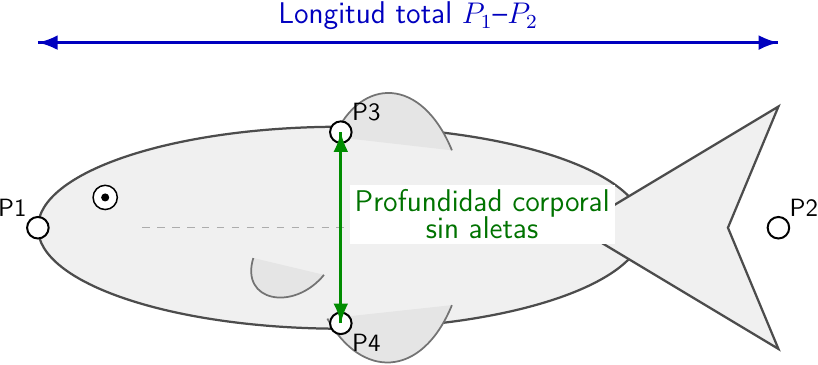
\includegraphics[width=0.8\textwidth]{fig2_2_puntos.png}
\fignota{Elaboración propia.}
\end{figure}

Las medidas tomadas con calibre sobre las réplicas constituyen la referencia contra la cual se evalúa cada estimación. Esta referencia también tiene error, que depende de la resolución del instrumento, de la ubicación de los puntos anatómicos y de la repetibilidad del procedimiento. Por ese motivo se utilizan las mismas definiciones anatómicas en la medición física y en la digital.

\subsubsection{Exactitud, repetibilidad e incertidumbre de la referencia}

La medición manual de un pez no da siempre el mismo resultado: varía entre operadores y entre repeticiones de un mismo operador. Influyen la ubicación de cada punto, la presión del instrumento, la posición del objeto, la resolución del calibre y la experiencia de quien mide \parencite{Petrtyl2014}. El valor manual, por lo tanto, no es un valor exento de incertidumbre, sino una referencia obtenida con un procedimiento controlado.

La exactitud de la referencia indica cuán cerca está del valor real de la magnitud medida; la repetibilidad, cuánto se dispersan las lecturas tomadas en las mismas condiciones. La resolución y la exactitud declaradas del instrumento, la variación entre repeticiones y la elección de los puntos anatómicos agregan incertidumbre a la referencia, y esta debe tenerse presente antes de extraer conclusiones de diferencias pequeñas entre el valor manual y el estimado.

\subsection{Formación de imágenes en medios acuáticos}

\subsubsection{Modelo geométrico convencional de cámara}

El modelo de cámara estenopeica, o \emph{pinhole}, representa la cámara como una caja con un orificio diminuto, de modo que todos los rayos de la escena pasan por ese único punto, el centro de proyección, antes de llegar al plano de la imagen. Con este modelo, la relación entre un punto del espacio, expresado en coordenadas del mundo, y su proyección en la imagen se escribe como \parencite{Hartley2004,Zhang2000}:
\begin{equation}
\lambda \begin{bmatrix} u \\ v \\ 1 \end{bmatrix} = \mathbf{K}\,[\mathbf{R} \mid \mathbf{t}]\begin{bmatrix} X_w \\ Y_w \\ Z_w \\ 1 \end{bmatrix},
\label{eq:pinhole}
\end{equation}
donde $(X_w, Y_w, Z_w)$ son las coordenadas del punto en el sistema del mundo, $(u, v)$ son sus coordenadas en la imagen y $\lambda$ es un factor de escala ligado a la profundidad del punto.

La matriz $\mathbf{K}$ reúne los parámetros intrínsecos, que describen las características internas de la cámara:
\begin{equation}
\mathbf{K} = \begin{bmatrix} f_x & \gamma & c_x \\ 0 & f_y & c_y \\ 0 & 0 & 1 \end{bmatrix},
\label{eq:K}
\end{equation}
donde $f_x$ y $f_y$ son las distancias focales en píxeles, $(c_x, c_y)$ es el punto principal y $\gamma$ recoge una posible falta de perpendicularidad entre los ejes del sensor. Estos parámetros transforman coordenadas de la cámara en coordenadas de la imagen y, en principio, no dependen de la ubicación de la cámara \parencite{Hartley2004}.

Los parámetros extrínsecos, la matriz de rotación $\mathbf{R}$ y el vector de traslación $\mathbf{t}$, describen la posición y la orientación de la cámara. Juntos definen la transformación rígida que lleva las coordenadas del mundo a las de la cámara \parencite{Hartley2004,Zhang2000}.

El modelo \emph{pinhole} es una idealización y no incluye la distorsión que introduce la lente. En una cámara convencional se lo completa con coeficientes de distorsión radial y tangencial. Cuando la imagen se forma a través de interfaces aire--vidrio--agua, en cambio, la refracción modifica además la dirección de los rayos y puede invalidar el supuesto de un único centro de proyección \parencite{Treibitz2012,Seegraber2025}.

\subsubsection{Distorsión óptica producida por la lente}

Una lente real no se comporta como el orificio ideal, sino que desplaza ligeramente la posición de los puntos en la imagen. La formulación habitual describe estos desplazamientos con una componente radial y otra tangencial \parencite{Brown1966,Weng1992}.

Sean $(x, y)$ las coordenadas normalizadas que tendría un punto con una proyección ideal, y sea
\begin{equation}
r^2 = x^2 + y^2,
\end{equation}
donde $r$ es la distancia del punto al eje óptico en el plano normalizado. Las coordenadas distorsionadas, $(x_d, y_d)$, resultan
\begin{equation}
\begin{aligned}
x_d &= x\left(1 + k_1 r^2 + k_2 r^4 + k_3 r^6\right) + 2p_1 xy + p_2\left(r^2 + 2x^2\right),\\
y_d &= y\left(1 + k_1 r^2 + k_2 r^4 + k_3 r^6\right) + p_1\left(r^2 + 2y^2\right) + 2p_2 xy.
\end{aligned}
\label{eq:distorsion}
\end{equation}

Los coeficientes $k_1$, $k_2$ y $k_3$ describen la componente radial. Su efecto crece con la distancia $r$ y se manifiesta principalmente hacia los bordes de la imagen, donde las líneas rectas se curvan en forma de barril o de cojín. Los coeficientes $p_1$ y $p_2$ describen la componente tangencial, o de descentrado, que aparece cuando los elementos de la lente, el eje óptico y el sensor no están perfectamente alineados, y que por ese motivo puede desplazar los puntos de forma asimétrica según la zona de la imagen.

Todos estos coeficientes pertenecen al conjunto cámara--lente. En una calibración convencional se estiman junto con los parámetros intrínsecos, minimizando el error de reproyección bajo el supuesto de una cámara central, es decir, \emph{pinhole} \parencite{Zhang2000}. Con esa compensación la cámara se aproxima a la proyección que produciría una cámara ideal sin distorsión.

La refracción en un puerto plano es un fenómeno distinto. Al atravesar las interfaces aire--vidrio--agua, los rayos dejan de converger, en general, en un único punto, y el sistema se convierte en una cámara axial no central, cuya geometría depende de la orientación y la posición de las interfaces, de sus espesores y de los índices de refracción de cada medio \parencite{Agrawal2012,JordtSedlazeck2012}.

\subsubsection{Refracción en la interfaz aire--vidrio--agua}

Un rayo de luz se desvía al pasar de un medio a otro con distinto índice de refracción. En una interfaz entre dos medios, la ley de Snell relaciona el ángulo de incidencia $\theta_1$, el ángulo refractado $\theta_2$ y los índices de refracción $n_1$ y $n_2$ \parencite{Hecht2017}:
\begin{equation}
n_1 \sin\theta_1 = n_2 \sin\theta_2 .
\label{eq:snell}
\end{equation}

Los ángulos se miden respecto de la normal de la interfaz. En el montaje utilizado, la luz que proviene del objeto atraviesa primero el agua, luego la pared transparente y por último el aire situado frente a la cámara; recorrido en sentido inverso, desde la cámara, el orden es aire, vidrio y agua. La ley de Snell se aplica en cada interfaz, teniendo en cuenta los índices, la orientación de las superficies y su geometría. Como señalan \textcite{Seegraber2025}, una carcasa o un puerto modifica el modelo de formación de la imagen, ya que el camino de cada rayo depende de la forma y la orientación del puerto, de la posición de la cámara respecto de él y de los medios que atraviesa.

\subsubsection{Modelo refractivo de puerto plano}
\label{sec:puerto-plano}

Un puerto plano se modela con dos interfaces paralelas: una entre el aire y la pared transparente, y otra entre la pared y el agua. Para seguir el rayo que corresponde a un píxel conviene recorrerlo desde la cámara hacia la escena. Por el principio de reversibilidad óptica, ese camino coincide con el que recorre la luz desde el objeto hasta la cámara, en sentido contrario \parencite{Agrawal2012,JordtSedlazeck2012}. La Figura~\ref{fig:2-3} muestra la geometría.

\begin{figure}[H]
\centering
\caption[Modelo refractivo de puerto plano]{Modelo refractivo de puerto plano. El centro de la cámara $C$ es el origen; las interfaces $\Pi_1$ (aire--vidrio) y $\Pi_2$ (vidrio--agua) son planos paralelos a distancias $d$ y $d + t_g$ de $C$, con normal común $\mathbf{n}_\pi$. El rayo de un píxel sale de $C$ con dirección $\mathbf{v}_a$, se refracta en $\mathbf{q}_1$ ($\mathbf{v}_g$), atraviesa el vidrio, se refracta de nuevo en $\mathbf{q}_2$ ($\mathbf{v}_w$) y recorre el agua según $\mathbf{X}(\lambda) = \mathbf{q}_2 + \lambda\,\mathbf{v}_w$ (ecuaciones~\ref{eq:q1} a~\ref{eq:rayo}). La línea punteada muestra dónde iría el rayo sin refracción.}
\label{fig:2-3}
\begin{tikzpicture}[scale=0.92,>=Stealth,font=\small]
  % medios
  \fill[gray!22] (4.0,-0.6) rectangle (4.6,5.2);
  \fill[cyan!7]  (4.6,-0.6) rectangle (8.8,5.2);
  \draw[gray!60!black,thick] (4.0,-0.6) -- (4.0,5.2);
  \draw[gray!60!black,thick] (4.6,-0.6) -- (4.6,5.2);
  \node[gray!50!black,above] at (2.0,5.2) {aire, $\mu_a$};
  \node[gray!50!black,above] at (4.3,5.2) {vidrio, $\mu_g$};
  \node[gray!50!black,above] at (7.8,5.2) {agua, $\mu_w$};
  \node[gray!60!black,below] at (4.0,-0.6) {$\Pi_1$};
  \node[gray!60!black,below] at (4.6,-0.6) {$\Pi_2$};
  % eje óptico y normal
  \draw[dashed,gray] (0,0) -- (8.8,0);
  \draw[->,thick] (4.0,0) -- (5.3,0) node[below right=-2pt] {$\mathbf{n}_\pi$};
  % centro de cámara
  \fill (0,0) circle (2.2pt); \node[below left] at (0,0) {$C$};
  % rayo
  \coordinate (q1) at (4.0,2.80);
  \coordinate (q2) at (4.6,3.05);
  \coordinate (X)  at (7.9,4.62);
  \draw[gray,dotted,thick] (q1) -- ++(35:2.6) node[above=2pt,font=\footnotesize,align=center] {rayo sin\\refracción};
  \draw[metC,very thick,->] (0,0) -- (q1);
  \draw[metC,very thick,->] (q1) -- (q2);
  \draw[metC,very thick,->] (q2) -- (X);
  \fill[metC] (q1) circle (2pt); \fill[metC] (q2) circle (2pt); \fill[metC] (X) circle (2.2pt);
  \node[metC,left=3pt] at (q1) {$\mathbf{q}_1$};
  \node[metC,right=3pt] at (q2) {$\mathbf{q}_2$};
  \node[metC,below right=-2pt] at (X) {$\mathbf{X}(\lambda)=\mathbf{q}_2+\lambda\,\mathbf{v}_w$};
  % direcciones
  \node[metC,above left=-2pt,rotate=35] at (2.1,1.5) {$\mathbf{v}_a$};
  \node[metC,above=1pt,rotate=22] at (4.3,2.95) {$\mathbf{v}_g$};
  \node[metC,above left=-2pt,rotate=25] at (6.4,3.9) {$\mathbf{v}_w$};
  % cotas
  \draw[<->] (0,-0.35) -- (4.0,-0.35) node[midway,below] {$d$};
  \draw[<->] (4.0,4.75) -- (4.6,4.75) node[midway,above,font=\footnotesize] {$t_g$};
  \draw[<->] (0,-1.0) -- (4.6,-1.0) node[midway,below] {$d + t_g$};
\end{tikzpicture}
\fignota{Adaptado de \emph{A theory of multi-layer flat refractive geometry}, por A. Agrawal, S. Ramalingam, Y. Taguchi y V. Chari, 2012, \emph{2012 IEEE Conference on Computer Vision and Pattern Recognition}, pp. 3346--3353 (\url{https://doi.org/10.1109/CVPR.2012.6248073}).}
\end{figure}

Se toma el centro de proyección de la cámara como origen de coordenadas y se llama $\mathbf{n}_\pi$ al vector unitario normal a las interfaces, orientado desde la cámara hacia la escena. La cara exterior de la pared (del lado del aire, $\Pi_1$) y la cara interior (del lado del agua, $\Pi_2$) se escriben como
\begin{align}
\Pi_1 &: \mathbf{n}_\pi^{\mathsf{T}}\mathbf{X} = d, \label{eq:pi1}\\
\Pi_2 &: \mathbf{n}_\pi^{\mathsf{T}}\mathbf{X} = d + t_g, \label{eq:pi2}
\end{align}
donde $d$ es la distancia perpendicular entre el centro de la cámara y la primera interfaz, y $t_g$ es el espesor de la pared. Esta representación supone dos superficies planas, paralelas y con la misma normal.

Para un punto de la imagen en coordenadas homogéneas, $\tilde{\mathbf{p}} = (u, v, 1)^{\mathsf{T}}$, ya corregido de la distorsión de la lente, la dirección unitaria del rayo en el aire es
\begin{equation}
\mathbf{v}_a = \frac{\mathbf{K}^{-1}\tilde{\mathbf{p}}}{\lVert \mathbf{K}^{-1}\tilde{\mathbf{p}} \rVert},
\label{eq:va}
\end{equation}
donde $\mathbf{K}$ es la matriz de parámetros intrínsecos de la cámara. El rayo toca la cara exterior del puerto en
\begin{equation}
\mathbf{q}_1 = \frac{d}{\mathbf{n}_\pi^{\mathsf{T}}\mathbf{v}_a}\,\mathbf{v}_a .
\label{eq:q1}
\end{equation}

Para calcular la desviación del rayo al pasar de un medio $i$ a un medio $j$ se utiliza la forma vectorial de la ley de Snell. Si $\mathbf{v}_i$ es la dirección unitaria incidente y $\eta_{ij} = \mu_i/\mu_j$ es el cociente entre los índices de refracción, entonces
\begin{equation}
\mathcal{R}(\mathbf{v}_i; \mu_i, \mu_j, \mathbf{n}_\pi) = \eta_{ij}\left(\mathbf{v}_i - (\mathbf{v}_i^{\mathsf{T}}\mathbf{n}_\pi)\,\mathbf{n}_\pi\right) + \sqrt{1 - \eta_{ij}^2\left(1 - (\mathbf{v}_i^{\mathsf{T}}\mathbf{n}_\pi)^2\right)}\;\mathbf{n}_\pi .
\label{eq:snell-vec}
\end{equation}

Con esta expresión, la dirección del rayo dentro de la pared transparente es
\begin{equation}
\mathbf{v}_g = \mathcal{R}(\mathbf{v}_a; \mu_a, \mu_g, \mathbf{n}_\pi),
\label{eq:vg}
\end{equation}
donde $\mu_a$ y $\mu_g$ son los índices de refracción del aire y del material de la pared. El rayo atraviesa entonces el espesor $t_g$ y sale del vidrio en
\begin{equation}
\mathbf{q}_2 = \mathbf{q}_1 + \frac{t_g}{\mathbf{n}_\pi^{\mathsf{T}}\mathbf{v}_g}\,\mathbf{v}_g .
\label{eq:q2}
\end{equation}

Una segunda aplicación de la ley de Snell, en la interfaz vidrio--agua, proporciona la dirección final del rayo dentro del agua:
\begin{equation}
\mathbf{v}_w = \mathcal{R}(\mathbf{v}_g; \mu_g, \mu_w, \mathbf{n}_\pi),
\label{eq:vw}
\end{equation}
donde $\mu_w$ es el índice de refracción del agua. Todos los puntos de la escena que pueden haber producido ese píxel se encuentran, por lo tanto, sobre el rayo
\begin{equation}
\mathbf{X}(\lambda) = \mathbf{q}_2 + \lambda\,\mathbf{v}_w, \qquad \lambda \geq 0 .
\label{eq:rayo}
\end{equation}
De manera equivalente, un punto $\mathbf{X}$ del espacio compatible con la observación debe cumplir
\begin{equation}
(\mathbf{X} - \mathbf{q}_2) \times \mathbf{v}_w = \mathbf{0}.
\label{eq:restriccion}
\end{equation}

Cada parámetro del puerto tiene un efecto identificable en la imagen. La normal $\mathbf{n}_\pi$ determina la orientación de las interfaces y, con ella, los ángulos de incidencia en cada aplicación de la ley de Snell. Si la normal coincide con el eje óptico, el efecto de la refracción es aproximadamente simétrico alrededor del centro de la imagen; si están desalineados, los rayos se desvían de manera distinta según su posición y esa simetría se pierde.

La distancia $d$ ubica la primera interfaz respecto del centro de la cámara y determina el punto $\mathbf{q}_1$ donde el rayo deja el aire. No modifica el ángulo que impone la ley de Snell, pero desplaza los puntos de intersección y, con ellos, la posición del rayo en el espacio. El espesor $t_g$ tiene un efecto similar, ya que determina la distancia que recorre el rayo dentro de la pared y la separación entre $\mathbf{q}_1$ y $\mathbf{q}_2$.

Los índices $\mu_a$, $\mu_g$ y $\mu_w$ actúan a través de sus cocientes y determinan la desviación del rayo en cada interfaz. Con dos superficies paralelas, el ángulo final del rayo respecto de la normal depende solo de los índices del primer y del último medio; aun así, el índice del vidrio y su espesor influyen en el desplazamiento lateral y en el punto por el que el rayo ingresa al agua.

Dado que cada píxel tiene su propio punto de partida $\mathbf{q}_2$ y su propia dirección $\mathbf{v}_w$, los rayos en el agua no necesariamente se cruzan en un único centro de proyección. Un sistema con interfaces planas y paralelas es, en general, una cámara axial no central, en la que cada rayo se mantiene en el plano formado por el rayo incidente y la normal del puerto \parencite{Agrawal2012}.

\paragraph{Aproximación de primer orden.} Cuando los rayos inciden de forma casi perpendicular al vidrio, la ecuación~\eqref{eq:snell-vec} puede linealizarse y el sistema se comporta como una cámara \emph{pinhole} cuya distancia efectiva al plano del objeto es
\begin{equation}
D(z) = d + \frac{t_g}{\mu_g} + \frac{z}{\mu_w},
\label{eq:Dz}
\end{equation}
donde $z$ es la profundidad del objeto detrás de la cara interior del vidrio. La magnificación de un objeto a profundidad $z$ es proporcional a $1/D(z)$, de modo que el tamaño aparente disminuye con la distancia. Esta relación no reemplaza al trazado completo, pero es suficiente para predecir el signo y el orden de magnitud del error de una escala tomada en el vidrio, así como el ancho del intervalo que produce el desconocimiento de la profundidad. En el Capítulo~\ref{cap:resultados} se contrastan ambas predicciones con los datos.

\subsubsection{Profundidad, inclinación y acortamiento aparente}

La posibilidad de recuperar medidas físicas a partir de una imagen depende de la ubicación relativa de la cámara, la pared transparente, el objeto y la referencia métrica. Detrás de una pared plana, la posición y el tamaño aparente del objeto cambian con su profundidad y con su ubicación en el campo de visión \parencite{Hartley2004,Treibitz2012}.

Para que una medida observada represente adecuadamente al objeto, su plano lateral debe ser aproximadamente paralelo a la pared. Si el objeto gira fuera de ese plano, sus dimensiones proyectadas se acortan. Algo similar ocurre si el eje longitudinal se inclina, porque cambia la orientación de la medida en la imagen y resulta más difícil ubicar los puntos anatómicos.

Una escala obtenida de una referencia visual solo puede trasladarse al objeto si ambos se encuentran en condiciones geométricas equivalentes. Si el marcador y la réplica están a profundidades distintas, la perspectiva y la refracción les asignan escalas aparentes distintas \parencite{Monkman2019}, como muestra la Figura~\ref{fig:2-5}.

\begin{figure}[H]
\centering
\caption[Escala aparente de un marcador según su profundidad]{Un marcador fijo en el vidrio y una réplica situada a profundidad $z$ se observan con magnificaciones distintas: la escala del marcador (rojo) no se transfiere a la réplica (verde). Un marcador coplanar con la réplica (naranja) comparte su magnificación.}
\label{fig:2-5}
\begin{tikzpicture}[scale=0.9,>=Stealth,font=\small]
  % vidrio
  \fill[gray!25] (2.0,-0.3) rectangle (2.3,3.3);
  \node[gray!70!black,above] at (2.15,3.3) {vidrio};
  \fill[cyan!8] (2.3,-0.3) rectangle (10.6,3.3);
  % cámara
  \node[draw,fill=white,minimum width=0.9cm,minimum height=0.6cm] (cam) at (0.2,1.5) {};
  \fill (0.65,1.5) circle (1.5pt);
  \node[below] at (0.2,1.2) {cámara};
  % marcador en el vidrio
  \draw[very thick,metA] (2.35,1.0) -- (2.35,2.0);
  \node[metA,left,align=right] at (1.95,2.5) {marcador\\en el vidrio};
  % marcador coplanar y pez
  \draw[very thick,metAp] (6.2,0.5) -- (6.2,1.5);
  \draw[very thick,metC] (6.2,1.7) -- (6.2,2.9);
  \node[metAp,right,align=left] at (6.3,1.0) {marcador\\coplanar};
  \node[metC,right] at (6.3,2.3) {réplica (LT)};
  % rayos extremos del marcador en vidrio
  \draw[metA] (0.65,1.5) -- (2.35,1.0);
  \draw[metA] (0.65,1.5) -- (2.35,2.0);
  % rayos de la réplica: aire hasta vidrio, luego quebrados
  \draw[metC] (0.65,1.5) -- (2.0,1.62) -- (2.3,1.645) -- (6.2,1.7);
  \draw[metC] (0.65,1.5) -- (2.0,2.33) -- (2.3,2.40) -- (6.2,2.9);
  % anotación
  \draw[<->] (2.3,-0.15) -- (6.2,-0.15) node[midway,below] {$z$ (profundidad desconocida)};
  \node[align=left,font=\footnotesize,anchor=west] at (8.35,1.0) {misma longitud,\\distinto tamaño\\aparente};
\end{tikzpicture}
\fignota{Elaboración propia.}
\end{figure}

La ubicación de la cámara, el tamaño y el material del tanque, las distancias de trabajo, la posición del marcador y las tolerancias de postura, inclinación y diferencia de profundidad son decisiones del diseño experimental. El Capítulo~\ref{cap:metodologia} detalla estos valores y el esquema del montaje.

\subsubsection{Profundidad conocida y profundidad desconocida}
\label{sec:z-desconocida}

La profundidad $z$ es la distancia entre el objeto y la referencia geométrica del montaje, medida desde la cara interna del vidrio o en el sistema de coordenadas de la calibración. Se considera conocida cuando un soporte fija y mide la posición de la réplica. En ese caso, cada rayo se interseca con el plano del objeto, se obtiene una estimación puntual y es posible comparar A, \Aprime, B y C contra la referencia física.

Se considera desconocida cuando una sola imagen no permite determinar a qué distancia del vidrio se encuentra el pez. En ese caso se evalúa C sobre todo el rango físicamente posible, $z \in [z_{\min}, z_{\max}]$. Si $L(z)$ es la longitud que se obtiene al suponer la profundidad $z$, el intervalo geométrico es
\begin{equation}
\IL = \Big[\min_{z \in [z_{\min}, z_{\max}]} L(z),\ \max_{z \in [z_{\min}, z_{\max}]} L(z)\Big].
\label{eq:IL}
\end{equation}

La forma abreviada $[L(z_{\min}), L(z_{\max})]$ solo es equivalente si $L(z)$ es monótona en el rango. En la aproximación de primer orden de la ecuación~\eqref{eq:Dz}, $L(z)$ es proporcional a $D(z)$ y, por lo tanto, crece con $z$; en el Capítulo~\ref{cap:resultados} se verifica con el trazado completo. El intervalo expresa únicamente la incertidumbre debida a la profundidad desconocida. No incluye los errores de calibración, de postura, de marcado manual ni de la referencia de calibre, que se informan por separado (Secciones~\ref{sec:calibraciones} y~\ref{sec:sensibilidad} y Tabla~\ref{tab:replicas}); la repetibilidad del marcado no se cuantificó. No debe interpretarse como un intervalo de confianza.

\subsubsection{Calibración y corrección refractiva}

CalibMar, el software de \textcite{Seegraber2025}, calibra cámaras y carcasas con puertos planos o en cúpula, y estima tanto los parámetros intrínsecos como los de la geometría refractiva. En este trabajo opera como antecedente instrumental, ya que los perfiles de calibración se obtuvieron con la rutina \texttt{calibrateCamera} de OpenCV \parencite{Zhang2000}, y la ruta C utiliza el trazado de rayos implementado en la aplicación desarrollada en este trabajo (Sección~\ref{sec:metodos}).

Para medir el efecto geométrico se aplican las cuatro rutas, A, \Aprime, B y C, a la misma escena. Si la imagen, el criterio de marcado, los puntos anatómicos y la referencia física se mantienen fijos, las diferencias de error pueden atribuirse con mayor claridad al tratamiento geométrico. La salida de una herramienta de calibración no es, por sí misma, una «corrección refractiva», ni puede convertirse sin verificación en coeficientes de distorsión de lente. La ruta C requiere parámetros, unidades, un sistema de coordenadas y un trazado coherentes con la geometría del montaje; por ese motivo se documentan los parámetros que consume, sus unidades y el sistema de coordenadas que utiliza.

\subsection{Estrategias de conversión métrica A, \Aprime, B y C}
\label{sec:rutas}

El experimento compara cuatro rutas geométricas aplicadas a los mismos puntos de cada imagen. La Figura~\ref{fig:2-4} las presenta de forma comparada.

\begin{figure}[H]
\centering
\caption[Las cuatro rutas de conversión métrica lado a lado]{Las cuatro rutas de conversión métrica sobre la misma escena. A toma la escala de un marcador en el vidrio y supone rayos rectos; \Aprime{} rectifica el plano del marcador coplanar con la réplica; B usa una cámara \emph{pinhole} con parámetros efectivos ajustados bajo el agua; C traza cada rayo a través de aire, vidrio y agua.}
\label{fig:2-4}
\begin{tikzpicture}[scale=0.6,>=Stealth,font=\scriptsize]
\foreach \x/\lab/\col/\txt in {0/A/metA/{escala del marcador\\en el vidrio},
                               6.4/\Aprime/metAp/{homografía del marcador\\coplanar con la réplica},
                               12.8/B/metB/{pinhole efectivo\\calibrado bajo el agua},
                               19.2/C/metC/{rayo refractado dos veces\\(puerto plano)}}{
  \begin{scope}[shift={(\x,0)}]
    \fill[gray!25] (1.6,0) rectangle (1.85,3.6);
    \fill[cyan!8] (1.85,0) rectangle (5.6,3.6);
    \node[draw,fill=white,minimum width=0.6cm,minimum height=0.45cm] at (0.3,1.8) {};
    \fill (0.6,1.8) circle (1.2pt);
    \draw[very thick,metC] (4.6,1.2) -- (4.6,2.6);
    \node[\col,font=\bfseries\small] at (2.8,4.1) {\lab};
    \node[align=center,font=\scriptsize] at (2.8,-0.55) {\txt};
  \end{scope}
}
% A: marcador en vidrio y rayos rectos
\draw[very thick,metA] (1.9,1.5) -- (1.9,2.1);
\draw[metA,dashed] (0.6,1.8) -- (4.6,1.2); \draw[metA,dashed] (0.6,1.8) -- (4.6,2.6);
% A': marcador junto a la réplica
\draw[very thick,metAp] (6.4+4.2,0.9) -- (6.4+4.2,1.5);
\draw[metAp,dashed] (6.4+0.6,1.8) -- (6.4+4.6,1.2); \draw[metAp,dashed] (6.4+0.6,1.8) -- (6.4+4.6,2.6);
% B: pinhole recto con damero
\foreach \i in {0,1,2}{\foreach \j in {0,1}{\fill[black!60] (12.8+2.3+\i*0.22,0.4+\j*0.22) rectangle ++(0.22,0.22);}}
\draw[metB] (12.8+0.6,1.8) -- (12.8+4.6,1.2); \draw[metB] (12.8+0.6,1.8) -- (12.8+4.6,2.6);
% C: rayos quebrados
\draw[metC] (19.2+0.6,1.8) -- (19.2+1.6,1.62) -- (19.2+1.85,1.6) -- (19.2+4.6,1.2);
\draw[metC] (19.2+0.6,1.8) -- (19.2+1.6,2.3) -- (19.2+1.85,2.34) -- (19.2+4.6,2.6);
\end{tikzpicture}
\fignota{Elaboración propia.}
\end{figure}

\begin{description}
  \item[A: escala directa en el vidrio.] El marcador ArUco queda pegado a la pared y su tamaño conocido convierte píxeles en milímetros. Constituye la línea de base más realista, la que emplearía cualquier usuario con una cámara y un marcador, pero está afectada por el paralaje: si la réplica se encuentra a otra profundidad, su escala aparente es distinta.
  \item[\Aprime: escala aproximadamente coplanar.] El marcador se coloca en el mismo plano de profundidad que la réplica, dentro de la tolerancia que fija la metodología. Esta ruta permite medir cuánto del error de A se debe a la separación entre marcador y objeto. Como rectifica el plano con una homografía, la diferencia entre A y \Aprime{} combina dos efectos: la coplanaridad y la corrección de perspectiva del plano del marcador.
  \item[B: cámara \emph{pinhole} calibrada bajo el agua.] Calibrar la cámara con un patrón visto a través del mismo sistema aire--vidrio--agua compensa la refracción de forma implícita: el ajuste elige parámetros intrínsecos y coeficientes de distorsión efectivos que minimizan el error de reproyección en la zona que cubren las imágenes de calibración. Esta calibración se realizó en la posición más cercana al vidrio y el error se estudió según la separación respecto de esa zona. La parametrización no reproduce la geometría no central de un puerto plano, pero puede aproximarla adecuadamente si se mide a distancias similares a las de la calibración \parencite{JordtSedlazeck2012,Treibitz2012,Shortis2015}. La limitación es que la compensación necesaria cambia con la distancia entre la cámara y el punto observado, de modo que un único conjunto de parámetros \emph{pinhole} no describe con la misma calidad objetos a distintas profundidades. Las simulaciones de \textcite{Rofallski2022} muestran que la calibración implícita funciona mejor cerca de la distancia de calibración y pierde exactitud al alejarse, y que se degrada aún más si el eje óptico no es perpendicular a la interfaz. La hipótesis H2 se apoya en ese comportamiento.
  \item[C: puerto plano explícito.] Cada rayo se sigue a través de las interfaces con la ley de Snell y las dimensiones se recuperan para una profundidad supuesta. Al recorrer una grilla de valores admisibles de $z$ se obtiene $L(z)$ y, cuando $z$ es desconocida, el intervalo geométrico $[\min_z L(z), \max_z L(z)]$. La ruta C no aísla la refracción como única causa, sino que incorpora el modelo completo de interfaces y la información de profundidad, lo que se tiene en cuenta al interpretar sus resultados.
\end{description}

El marcado manual, la imagen y la referencia física son los mismos para las cuatro rutas. En consecuencia, una diferencia entre métodos no puede atribuirse a una elección distinta de puntos ni a una imagen rectificada.

\subsection{Marcado manual de puntos anatómicos}

A diferencia de los trabajos de la Sección~\ref{sec:antecedentes}, que localizan los puntos anatómicos con redes neuronales, en este proyecto los cuatro puntos de cada captura se marcaron a mano sobre la imagen original, con un criterio anatómico fijo: $\mathbf{p}_1$ y $\mathbf{p}_2$ son los extremos de la longitud total, y $\mathbf{p}_3$ y $\mathbf{p}_4$, los de la profundidad corporal, sin incluir ninguna aleta.

Cada captura se marcó una sola vez y las mismas coordenadas se reutilizaron en A, \Aprime, B y C. Cada registro de medición conserva la réplica, la imagen, el operador, la fecha, el criterio aplicado y cualquier revisión. Un nuevo marcado, o una revisión independiente, permite estimar la repetibilidad del procedimiento, pero no lo convierte en una salida automática ni genera una nueva unidad experimental.

La incertidumbre de la ubicación manual de los puntos se separa de la incertidumbre geométrica por profundidad. Quedaron registrados los casos en que el contorno, la postura o la visibilidad de una aleta dificultaron la ubicación de un punto, así como el motivo de cada exclusión. Esta separación permite atribuir las diferencias entre A, \Aprime, B y C al tratamiento geométrico, dado que los puntos anatómicos son siempre los mismos.

\subsection{Recuperación de la escala física}

\subsubsection{Marcadores fiduciales ArUco}

Los marcadores ArUco son cuadrados con un borde negro y una matriz interna de celdas blancas y negras, cuyo patrón binario identifica a cada marcador. Al detectarlo, el algoritmo entrega su identificador y la posición de sus cuatro esquinas en la imagen. Si se conoce el tamaño real del marcador, esas esquinas vinculan la imagen con el mundo físico \parencite{GarridoJurado2014}.

En una escena frontal y casi plana, el tamaño aparente del marcador proporciona una escala local entre píxeles y milímetros. Si además se conocen los parámetros intrínsecos y de distorsión de la cámara, es posible estimar la pose del marcador respecto de ella. Por último, con las cuatro esquinas y sus posiciones conocidas en el plano puede construirse una homografía que rectifique ese plano. Las tres opciones no son equivalentes, porque la escala directa supone una magnificación casi uniforme, la pose depende del modelo de cámara y la homografía solo es válida para puntos situados en el mismo plano.

El diccionario, el identificador, el tamaño físico, la forma de cálculo elegida y las reglas para aceptar o descartar una detección son parámetros del sistema; el Capítulo~\ref{cap:metodologia} los documenta.

\subsubsection{Conversión entre píxeles y unidades físicas}

En una escena frontal y casi plana, el tamaño conocido del marcador proporciona una escala local. Sea $L_m$ la longitud física de su lado y sean $p_i$, con $i = 1, \ldots, 4$, las longitudes en píxeles de sus cuatro lados detectados. Cada una se calcula a partir de dos esquinas consecutivas:
\begin{equation}
p_i = \sqrt{(x_{i+1} - x_i)^2 + (y_{i+1} - y_i)^2},
\label{eq:lado}
\end{equation}
donde, para cerrar el contorno, se toma $(x_5, y_5) = (x_1, y_1)$.

\textcite{Monkman2019} estiman la cantidad de milímetros que representa un píxel promediando las escalas de los cuatro lados del marcador:
\begin{equation}
k = \frac{1}{4}\sum_{i=1}^{4}\frac{L_m}{p_i},
\label{eq:escala-monkman}
\end{equation}
donde $k$ queda en unidades físicas por píxel, por ejemplo mm/píxel. El promedio de los cuatro lados reduce la dependencia de una sola detección y absorbe las pequeñas diferencias entre las longitudes observadas en la imagen. La implementación utilizada divide el lado físico por el promedio de los cuatro lados en píxeles (Sección~\ref{sec:metodos}); para marcadores correctamente detectados, ambas variantes difieren en menos de una centésima de píxel.

Si $d_f$ es la distancia en píxeles entre dos puntos anatómicos, la longitud física estimada es
\begin{equation}
\hat{L}_f = k\,d_f .
\label{eq:Lf}
\end{equation}

\textcite{Monkman2019} emplearon este procedimiento para estimar la longitud total de peces con marcadores ArUco de tamaño conocido. El método supone que la magnificación es la misma en el marcador y en la región medida, lo que exige que ambos se encuentren aproximadamente en el mismo plano y con una orientación similar respecto de la cámara. Si están a distinta profundidad, aparece una diferencia de escala que esta relación no corrige.

Además, las esquinas del marcador y los puntos anatómicos deben expresarse en el mismo sistema de coordenadas y en la misma condición de corrección de la imagen. El Capítulo~\ref{cap:metodologia} indica en qué etapa del procesamiento se obtiene la escala y cómo se revisa el marcado.

\subsubsection{Homografía y perspectiva}

Una homografía es la transformación proyectiva que relaciona las coordenadas de un plano con las de su imagen, y se representa con una matriz de $3 \times 3$ \parencite{Hartley2004}. Rectifica únicamente el plano que la define: no recupera la posición espacial de los puntos situados fuera de ese plano, ni corrige la diferencia de escala que aparece cuando el marcador y el pez se encuentran a distinta profundidad. En presencia de refracción, además, la homografía es una aproximación, ya que puede ajustar adecuadamente las correspondencias del plano de referencia sin representar el camino de todos los rayos aire--vidrio--agua. La Sección~\ref{sec:metodos} presenta la homografía que usa \Aprime.

\subsection{Estimación y evaluación morfométrica}

Para evaluar una medición conviene distinguir tres propiedades. La exactitud indica cuán cerca se encuentra una estimación de la referencia física; la repetibilidad, cuánto se dispersan las repeticiones técnicas en las mismas condiciones; y la concordancia, si dos procedimientos producen valores comparables, lo que es una condición más exigente que la correlación \parencite{Bland1986,Lin1989}. Las tres propiedades se examinan sobre las mismas réplicas, con errores con signo y absolutos, métricas agregadas y análisis pareados.

La referencia manual se trata como una medición controlada que también tiene incertidumbre. Por ese motivo, MAE, RMSE y MAPE se interpretan como diferencias respecto de esa referencia, y el sesgo se utiliza para detectar tendencias sistemáticas. Las repeticiones de una misma réplica se resumieron antes de cualquier comparación inferencial, porque no son unidades experimentales independientes. Las definiciones, fórmulas, agregaciones y criterios de decisión están en el Capítulo~\ref{cap:metodologia}.

\subsubsection{Trazabilidad de la medición}

Para que una medición pueda reproducirse, cada resultado debe guardar, junto con el valor estimado, la imagen de origen, el modo de corrección, el perfil de calibración, el marcador usado, el protocolo de marcado, el operador, la unidad y las advertencias de calidad. Con esa información se puede reconstruir el camino completo, desde la captura hasta la comparación con la referencia, y determinar si un error proviene de la adquisición, la corrección, el marcado o la conversión métrica.

Los datos mínimos que entrega cada medición, la estructura del archivo JSON y las evidencias que se conservan para su inspección son decisiones de diseño e implementación. El Capítulo~\ref{cap:metodologia} las define y describe la trazabilidad efectiva entre los datos de entrada, los resultados y las evidencias.

\section{Marco conceptual}
\label{sec:conceptual}

Esta sección establece el sentido con que se emplean los términos principales del trabajo. Las definiciones resumen lo desarrollado en el marco referencial y en el Capítulo~\ref{cap:metodologia}.

\begin{description}
  \item[Morfometría.] Medición de las dimensiones y de la forma externa del cuerpo de un organismo. En este trabajo se reduce a dos medidas: la longitud total y la profundidad corporal.
  \item[Punto anatómico.] Lugar del cuerpo que puede ubicarse de forma repetible en la réplica y en la imagen. Se utilizan cuatro, de $\mathbf{p}_1$ a $\mathbf{p}_4$ (Sección~\ref{sec:puntos-def}).
  \item[Longitud total (LT).] Distancia entre el extremo anterior del hocico y el punto más posterior de la aleta caudal, medida sobre el eje longitudinal del pez.
  \item[Profundidad corporal (PC).] Distancia entre el perfil dorsal y el ventral en una misma sección transversal del cuerpo, sin incluir las aletas.
  \item[Réplica rígida.] Modelo de pez impreso en PLA cuyas dimensiones no cambian. Sus medidas con calibre son la referencia física de cada estimación.
  \item[Conversión métrica.] Transformación que lleva las coordenadas de un punto de la imagen, en píxeles, a milímetros. A, \Aprime, B y C son cuatro conversiones distintas (Sección~\ref{sec:rutas}).
  \item[Marcador ArUco.] Cuadrado de lado conocido con un código binario que un detector localiza automáticamente en la imagen \parencite{GarridoJurado2014}. Sus esquinas sirven como referencia de escala.
  \item[Homografía.] Transformación proyectiva entre dos planos, representada por una matriz de $3 \times 3$ \parencite{Hartley2004}. Corrige la perspectiva de los puntos que pertenecen al plano que la define.
  \item[Visión estéreo.] Técnica que recupera la posición tridimensional de un punto a partir de dos imágenes de la misma escena tomadas desde posiciones conocidas: la diferencia entre ambas imágenes permite triangular la distancia del punto a las cámaras \parencite{Hartley2004}. Requiere dos cámaras; en este trabajo se utiliza una sola.
  \item[Calibración de cámara.] Estimación de los parámetros intrínsecos de la cámara y de los coeficientes de distorsión de la lente a partir de imágenes de un patrón conocido, como un damero \parencite{Zhang2000}.
  \item[Modelo \emph{pinhole} efectivo.] Modelo de cámara \emph{pinhole} calibrado con el patrón bajo el agua. Incorpora de forma empírica el efecto de la refracción, sin representarla explícitamente, y es la base del método B.
  \item[Refracción e índice de refracción.] La refracción es el cambio de dirección de la luz al pasar de un medio a otro. El índice de refracción de cada medio determina la magnitud de la desviación, según la ley de Snell (ecuación~\ref{eq:snell}; \cite{Hecht2017}).
  \item[Puerto plano.] Pared transparente y plana que separa la cámara del agua. Se modela como dos interfaces paralelas, aire--vidrio y vidrio--agua (Sección~\ref{sec:puerto-plano}).
  \item[Profundidad $z$.] Distancia entre el plano de simetría de la réplica y la cara interna del vidrio. Es conocida cuando un soporte la fija, y desconocida cuando una sola imagen no permite determinarla (Sección~\ref{sec:z-desconocida}).
  \item[Intervalo geométrico $\IL$.] Rango de longitudes compatibles con todas las profundidades admisibles (ecuación~\ref{eq:IL}). Expresa la incertidumbre debida al desconocimiento de $z$ y no es un intervalo de confianza estadístico.
  \item[Exactitud y repetibilidad.] La exactitud indica cuán cerca está una medida del valor real; la repetibilidad, cuánto se dispersan las lecturas tomadas en las mismas condiciones.
\end{description}
